\documentclass[12pt, xcolor=dvipsnames]{article}

% should be defined before TIKZ! (for xcolor colors)
\usepackage[dvipsnames,prologue]{pstricks}

\usepackage{tikz}
\usetikzlibrary{shapes.geometric, arrows, positioning, decorations.markings}
\usetikzlibrary{fit}
\usepackage{microtype}
\usepackage{framed}
\usetikzlibrary{decorations.pathmorphing,calc,backgrounds}

\usepackage{graphicx}

\usepackage{amsmath}

\tikzset{
	pics/carc/.style args={#1:#2:#3}{
		code = {
			\draw[pic actions] (#1:#3) arc(#1:#2:#3);
		}
	}
}

\begin{document}

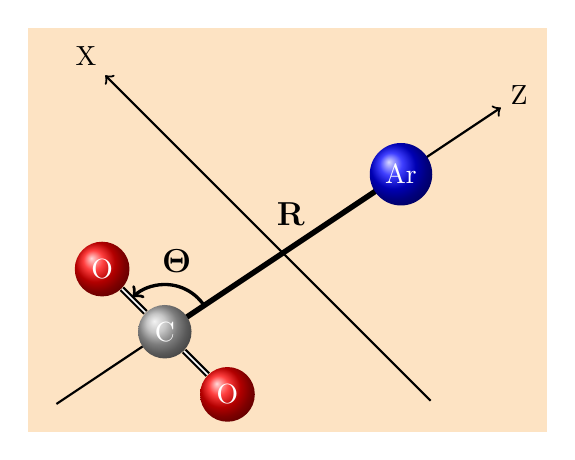
\begin{tikzpicture}
	[oxygen/.style={ball color = red, circle, text = white}, 
	carbon/.style={ball color = black!30, circle, text = white},
	argon/.style={ball color = blue, circle, text = white}]
	\node (z1) at (4.5, 3) {Z};
	\node (z2) at (-1.5, -1) {}
		edge [->, thick] (z1);
	
	\node (th1) at (3, 2) {};
	\node (th2) at (0, 0) {}
		edge [->, line width = 2pt] (th1);

	\node (r) at (1.6, 1.5) {$\large \textbf{R}$};
	\node (t) at (0.15, 0.9) {$\large \boldsymbol{\Theta}$};

	\node (theta1) at (0.4, -0.6) {};
	\node (theta2) at (0.58, 0.6) {};

	\draw[very thick, ->] pic[black]{carc=31:133:0.6cm};
	%\draw[very thick] pic[black]{carc=-45:30:0.7cm};

	\node (x1) at (-1, 3.5) {X};
	\node (x2) at (3.5, -1) {}
		edge [->, thick] (x1); 

	\newcommand{\CObondlength}{0.3cm}

	\node (carbon) [carbon] {C};
	\node (oxygen1) [oxygen, below right = \CObondlength and \CObondlength of carbon] {O}
		edge [double, thick] (carbon);
	\node (oxygen2) [oxygen, above left = \CObondlength and \CObondlength of carbon] {O}
		edge [double, thick] (carbon);
	\node[argon] (argon) at (3, 2) {Ar};
\begin{scope}[on background layer]
	\node [fill=BurntOrange!20,fit=(z1) (z2) (x1) (x2) (carbon) (oxygen1) (oxygen2)] {};
\end{scope}
\end{tikzpicture}


\end{document}

